\documentclass{ethpresentation}
\usepackage{multimedia}
% \setbeameroption{show notes on second screen} % use e.g. pympress to view

% Simple handout with just the slides
% "article" mode is better, but this might be useful in a pinch?
% \documentclass[handout]{ethpresentation}
% \usepackage{pgfpages}
% \pgfpagesuselayout{6 on 1}[a4paper,border shrink=5mm]

% Footnotes for sources without number
\let\svthefootnote\thefootnote
\NewDocumentCommand{\freefootnote}{m}{
  \let\thefootnote\relax%
  \footnotetext{#1}%
  \let\thefootnote\svthefootnote%
}

% Regular footnotes use letters
\renewcommand*{\thefootnote}{\fnsymbol{footnote}}

% Logo
\NewDocumentCommand{\magnethical}{}{\textnormal{\textsl{\textmd{\textsl{magn\textbf{ETH}ical}}}}}

% Notes:
% - Include challenges faced and overcome, so it's mentioned
% - Include lessons learned
% - estimate 2min per slide on average 
%  -> was a bit faster (~43min for 29 slides), took ~60min including demonstration


%%%%%%%%%%%%%%%%%%%%%%%%%%%%%%%%%%%%%%%%%%%%%%%%%%%%%%%%%%%%%%%%%%%%%%%%%%%%%%%
% Metadata
%%%%%%%%%%%%%%%%%%%%%%%%%%%%%%%%%%%%%%%%%%%%%%%%%%%%%%%%%%%%%%%%%%%%%%%%%%%%%%%

\title{\Huge\magnethical}
\subtitle{Master Thesis: Building a 25\,MHz NMR Spectrometer}
\date{\today}
\author{Maximilian Stabel}
\institute{ETH Zürich}


%%%%%%%%%%%%%%%%%%%%%%%%%%%%%%%%%%%%%%%%%%%%%%%%%%%%%%%%%%%%%%%%%%%%%%%%%%%%%%%
% Content
%%%%%%%%%%%%%%%%%%%%%%%%%%%%%%%%%%%%%%%%%%%%%%%%%%%%%%%%%%%%%%%%%%%%%%%%%%%%%%%

\begin{document}
\maketitle % show when people are walking in

% Attention Getter
\begin{frame}
    \centering
    \emph{\enquote{What I cannot create, I do not understand}}

    \vspace{\baselineskip}

    \hfill{}---Richard Feynman
    \note[item]{In the spirit of Richard Feynman... }
    \note[item]{My master thesis is about building an NMR spectrometer}
    \note[item]{I'm Max and I'll be your host for today}
    \note[item]{Speaking of understanding...}
\end{frame}

% Need / Motivation
\begin{frame}{There is not a lot of NMR research in the Global South}
    \centering
    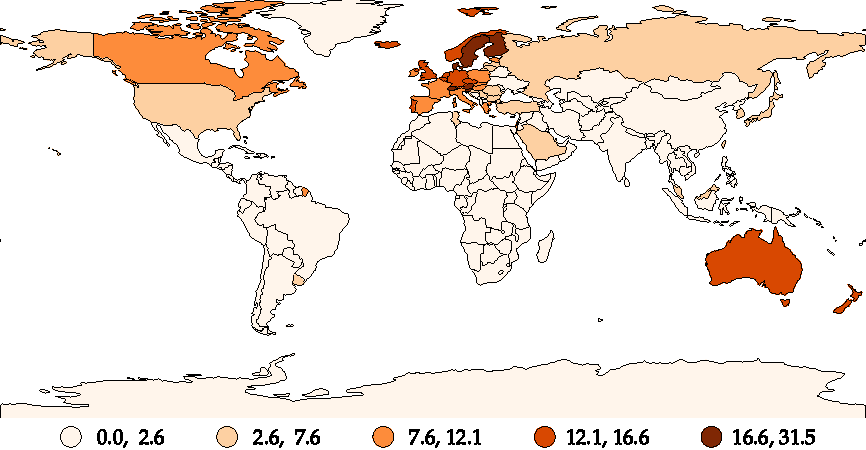
\includegraphics[height=0.8\textheight]{images/nmr-affiliations-per-million-people_naturalbreaks.pdf}

    \(\frac{\text{NMR publications}}{\text{million people}}\)
    \note[item]{Only publications, doesn't include use of NMR!}
    \note[item]{I'm Max and I'll talk about my master thesis: building a 25MHz NMR spectrometer}
\end{frame}
\note{Reminder: What is NMR spectrometer}

\begin{frame}{Nuclear Magnetic Resonance}
    \begin{itemize}
        \item Nuclei absorb radio waves at a certain frequency when inside a magnetic field
        \item The nuclei emit radio waves at that same frequency when excited this way
        \item \(f \sim{} B_0\) and surroundings
    \end{itemize}
\end{frame}

\note{
    \begin{itemize}
        \item You: Understanding for own experiments
        \item The better we know the better we can use
        \item Push NMR development --- better machines
        \item Transition: if not about you personally --- more globally: applications
    \end{itemize}
}


\begin{frame}{NMR is used across various fields}
    \note[item]{Some of you already know, but here are some reasons why NMR is useful}
    \begin{itemize}
        \item Research (Structure Analysis, Drug Discovery, \ldots)
        \item Medicine (Imaging, Diagnosis, \ldots)
        \item Industry (Process Control, Drug screening, \dots)
        \item Education (Quantum Mechanics, Quantum Computing, \ldots)
    \end{itemize}
\end{frame}


% Task / Main Message
% One sentence to remember if they remember only one
\begin{frame}[standout]
    \centering
    Build an accessible\\NMR spectrometer
    \note[item]{The goal of my thesis was...}
\end{frame}

% Preview
% Give short overview of main points to come
% DONT just list ("I will talk about ..., then about ...)
% Integrate with main message, include audience ("we")
% Introduction to NMR
% Will talk about the parts of the spectrometer
% Do a short demonstration..
% Show table of contents, without anything above (introduction, ...) and without conclusion/review/close
\begin{frame}{Preview}
    \tableofcontents
\end{frame}

% Main Body
% Remember to do transitions!
\section{The parts}
\begin{frame}{Our goal is to build an accessible NMR spectrometer}
    \centering
    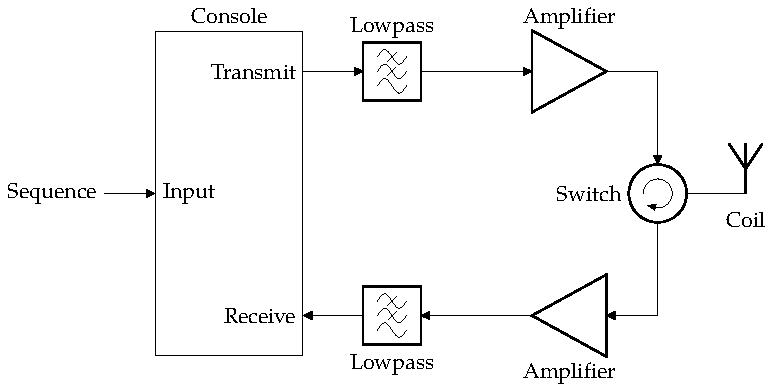
\includegraphics[width=0.9\textwidth]{block_diagram.pdf}
    % \begin{circuitikz}
    %   \ctikzset{bipoles/amp/width=0.9}
    %   \draw[nodes={align=center}]
    %   (0,0) coordinate(mid)

    %   % RP
    %   (mid) node[draw, minimum height=5.5cm, minimum width=2.5cm,label=Console](redpitaya){}
    %   (redpitaya.west) coordinate(inp) node[right]{Input}
    %   ($(redpitaya.east)!0.75!(redpitaya.north east)$) coordinate(rptx) node[left]{Transmit}
    %   ($(redpitaya.east)!0.75!(redpitaya.south east)$) coordinate(rprx) node[left]{Receive}

    %   % Computer
    %   (-3,0) node(seq){Sequence}
    %   (seq.east) -- (redpitaya.west) node[inputarrow]{} coordinate(console)

    %   % TX
    %   (rptx) to[lowpass,l=Lowpass,>] ++(3,0)
    %   to[amp,l=Amplifier,>] ++(3,0) coordinate(tx)

    %   % Circulator
    %   (mid -| tx) node[circulator,label={left:Switch}](circ){}
    %   (tx) -| (circ.n) node[inputarrow,rotate=270]{}

    %   % RX
    %   (rprx -| circ) coordinate(rx)
    %   (circ.s) |- (rx)
    %   (rx) to[amp,l=Amplifier,>] ++(-3,0)
    %   to[lowpass,l=Lowpass,>] ++(-3,0) node[inputarrow,rotate=180]{}

    %   % Probe
    %   (circ.e) -- ++(1,0)
    %   node[dinantenna](probe){}
    %   node[below=1ex]{Coil}
    %   ;
    % \end{circuitikz}
    \note[item]{Go through the parts left to right}
    \note[item]{Our switch only, others might include more analog processing}
\end{frame}

\begin{frame}{The console\\is a ready-made FPGA board\footnote{Red Pitaya SDRlab 122-16}}
    % \centering
    \vspace*{-1\baselineskip}
    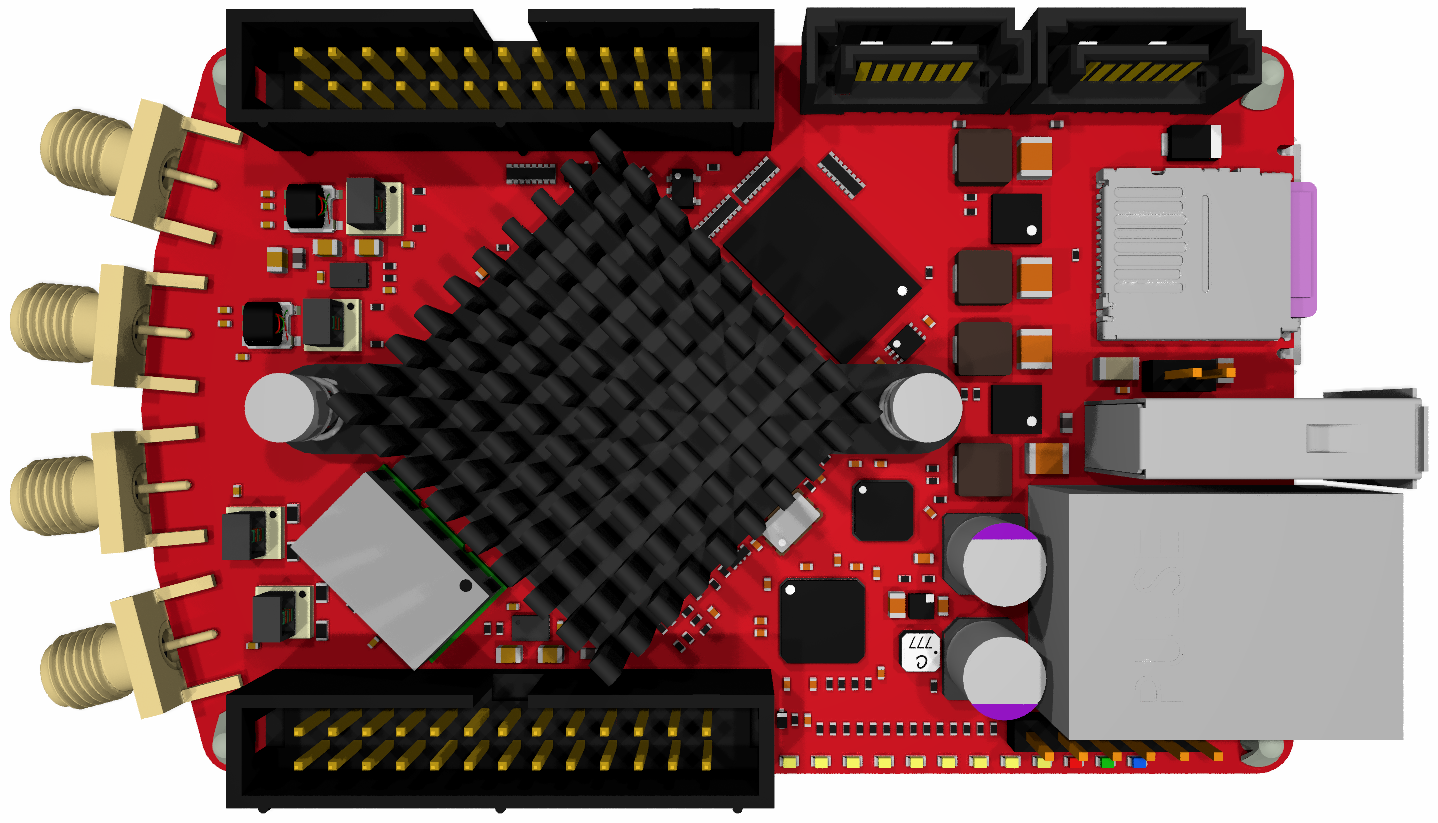
\includegraphics[height=0.7\textheight]{rp122-16.png}
    \begin{tikzpicture}[overlay, remember picture]
        \node[anchor=north east, inner sep=0] (block) at (current page.north east) {\colorbox{white}{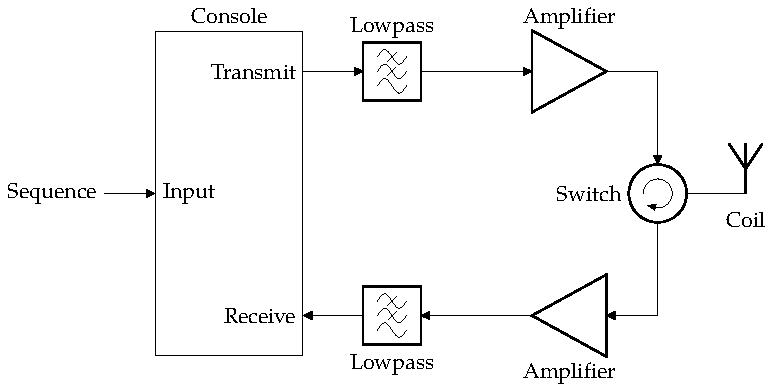
\includegraphics[width=6cm]{block_diagram.pdf}}};
        \draw[red, ultra thick, rounded corners] (block.south west) ++(0.1,0.2) rectangle ++(2.5,3);
    \end{tikzpicture}
    \note[item]{FPGA == programmable hardware, very fast}
    \note[item]{oversampling}
    \note[item]{CIC filter (decimation, low pass filter, moving average)}
    \note[item]{The signal needs to be filtered and then amplified: Next Slide}
\end{frame}

\begin{frame}{The power amplifier has two stages}
    \centering
    \vspace*{4\baselineskip}
    \begin{columns}
        \begin{column}{0.2\textwidth}
            \vspace*{2\baselineskip}
            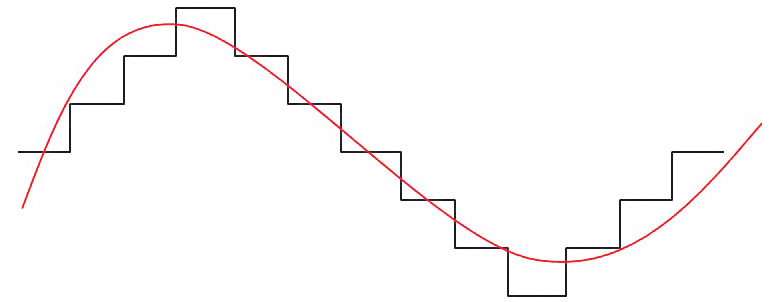
\includegraphics[width=\textwidth]{dds_wave.jpg}
        \end{column}
        \begin{column}{0.8\textwidth}
            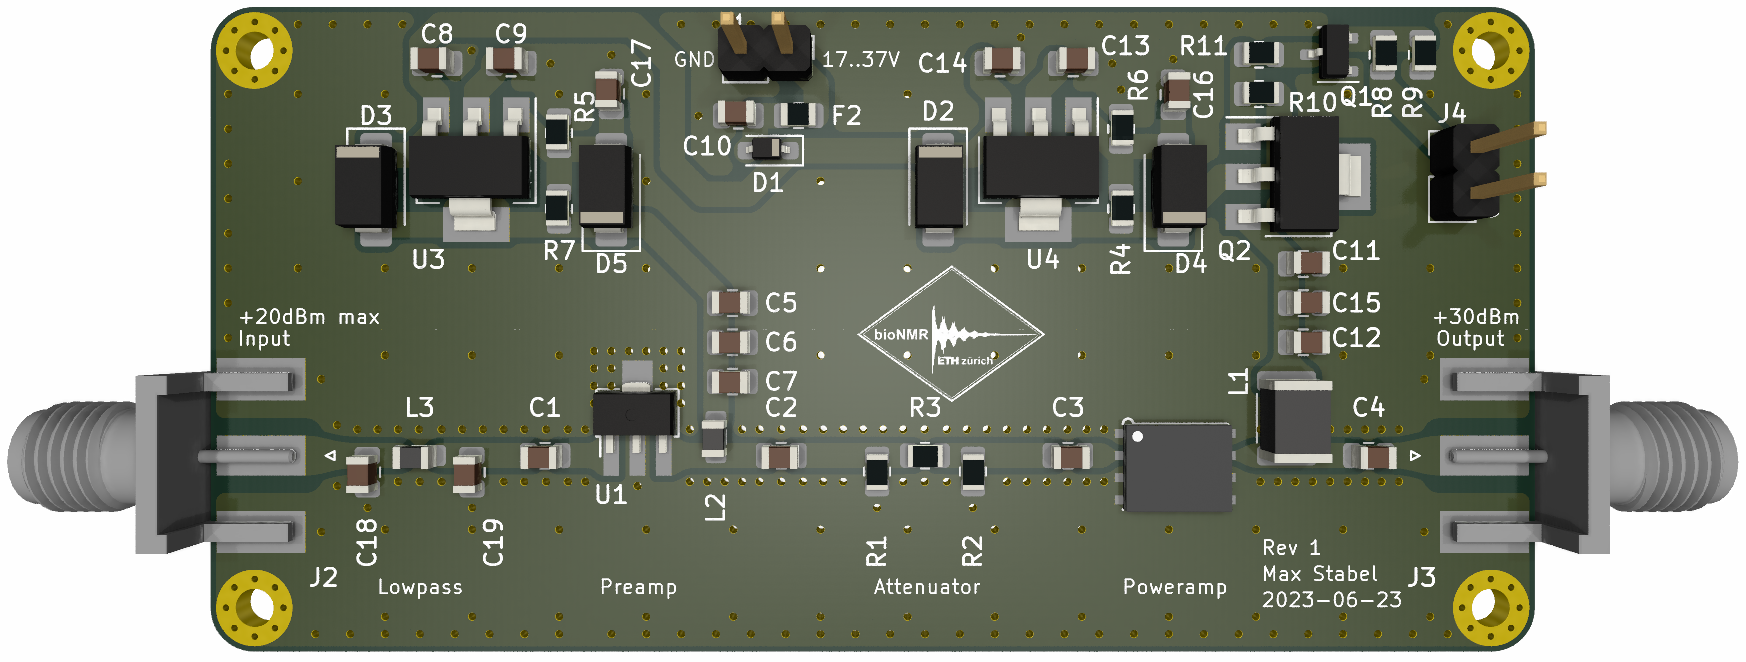
\includegraphics[width=\textwidth]{poweramp.png}
        \end{column}
    \end{columns}
    \begin{tikzpicture}[overlay, remember picture]
        \node[anchor=north east, inner sep=0] (block) at (current page.north east) {\colorbox{white}{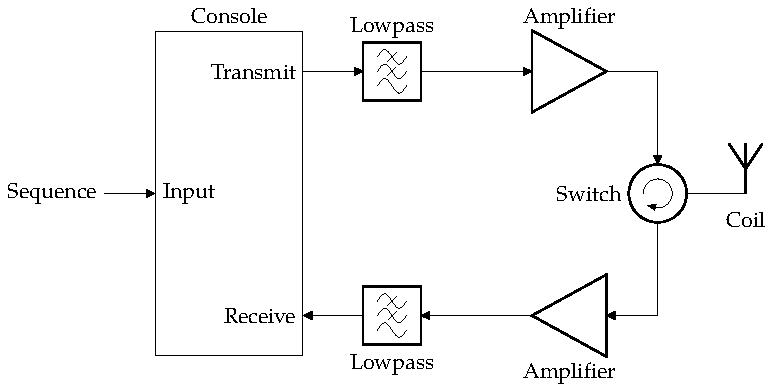
\includegraphics[width=6cm]{block_diagram.pdf}}};
        \draw[red, ultra thick, rounded corners] (block.south west) ++(2.7,2.2) rectangle ++(2.3,1);
    \end{tikzpicture}
    % 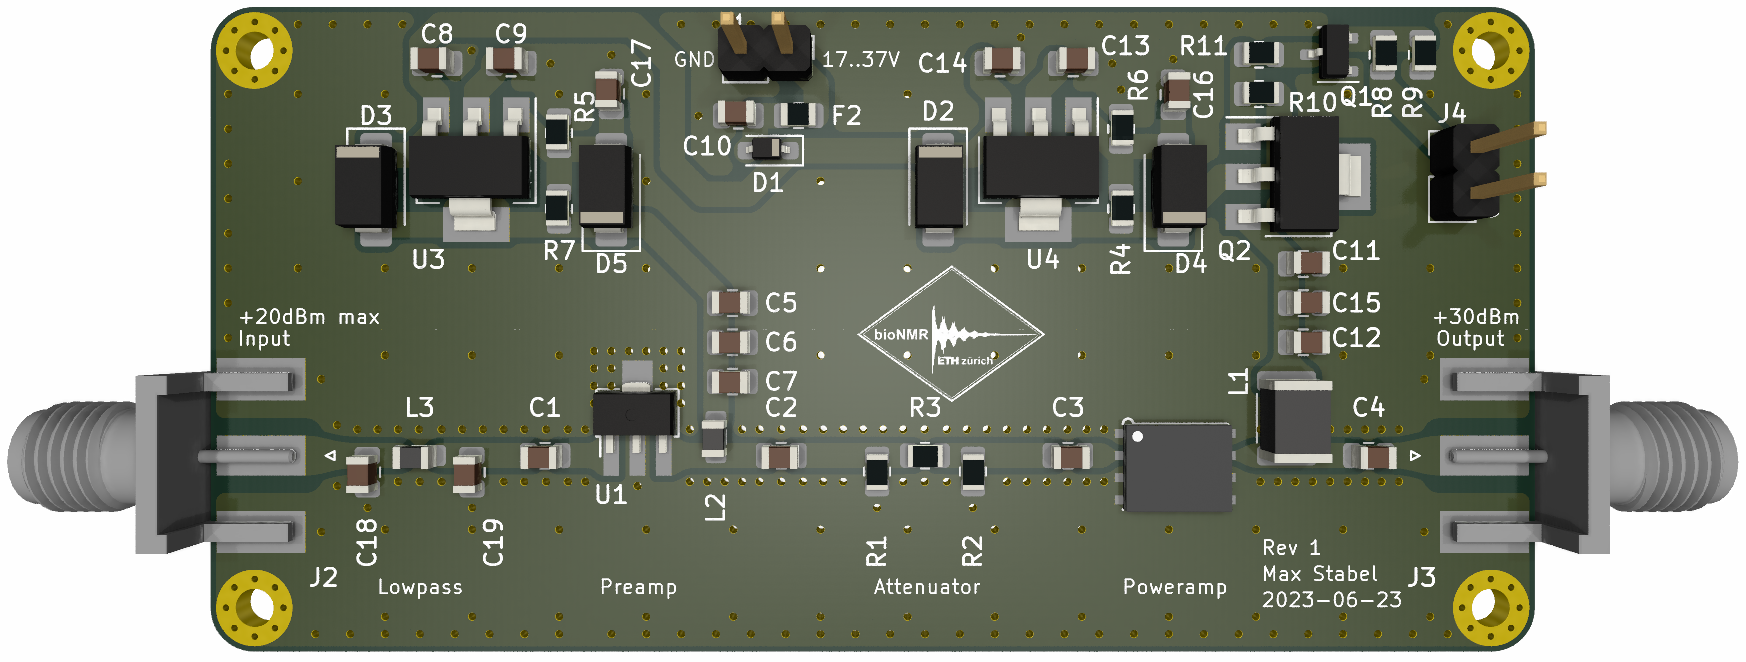
\includegraphics[width=0.9\textwidth]{poweramp.png}
    \note[item]{We want cheap, so using a simple is the obvious first approach}
    \note[item]{Unfortunately there's a lot to do:%
        \begin{itemize}
            \item Input/Output Impedance Matching
            \item Bias Tee
            \item DC coupling
            \item stability calculations
            \item feedback
            \item temperature compensation (current feedback)
        \end{itemize}
    }
    \note[item]{A complete amplifier is quite expensive}
    \note[item]{Solution: Use monolithic (integrated) amplifier}
    \note[item]{Take care of heat dissipation (Class-A)}
    \note[item]{dB is logarithmic unit}
\end{frame}

\begin{frame}{The low-noise amplifier had\\instability issues}
    \centering
    \vspace*{2\baselineskip}
    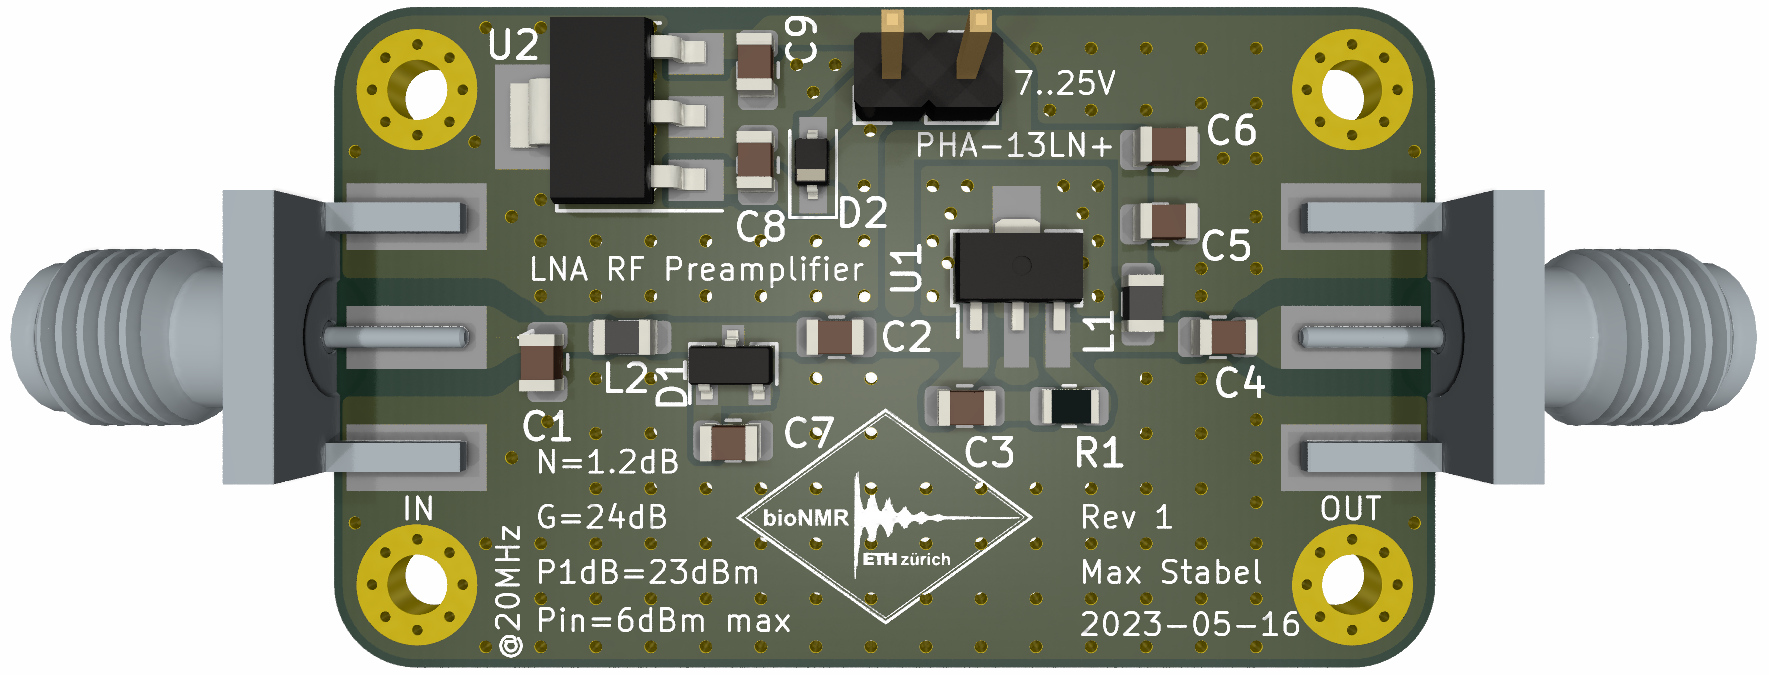
\includegraphics[width=0.9\textwidth]{preamp.png}
    \begin{tikzpicture}[overlay, remember picture]
        \node[anchor=north east, inner sep=0] (block) at (current page.north east) {\colorbox{white}{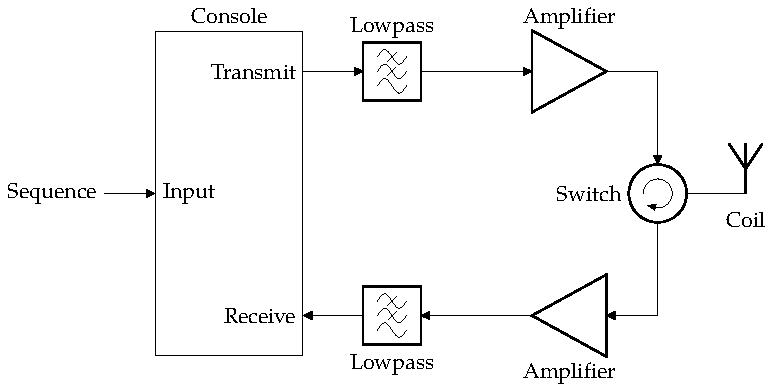
\includegraphics[width=6cm]{block_diagram.pdf}}};
        \draw[red, ultra thick, rounded corners] (block.south west) ++(4,0.1) rectangle ++(1,1);
    \end{tikzpicture}
    \note[item]{Low-noise }
    \note[item]{Feedback loop --- stray capacitance}
    \note[item]{Solution: Smaller housing, shorter loop}
    \note[item]{We need 3x for enough gain}
\end{frame}

\begin{frame}{We use a transistor-based active switch}
    \centering
    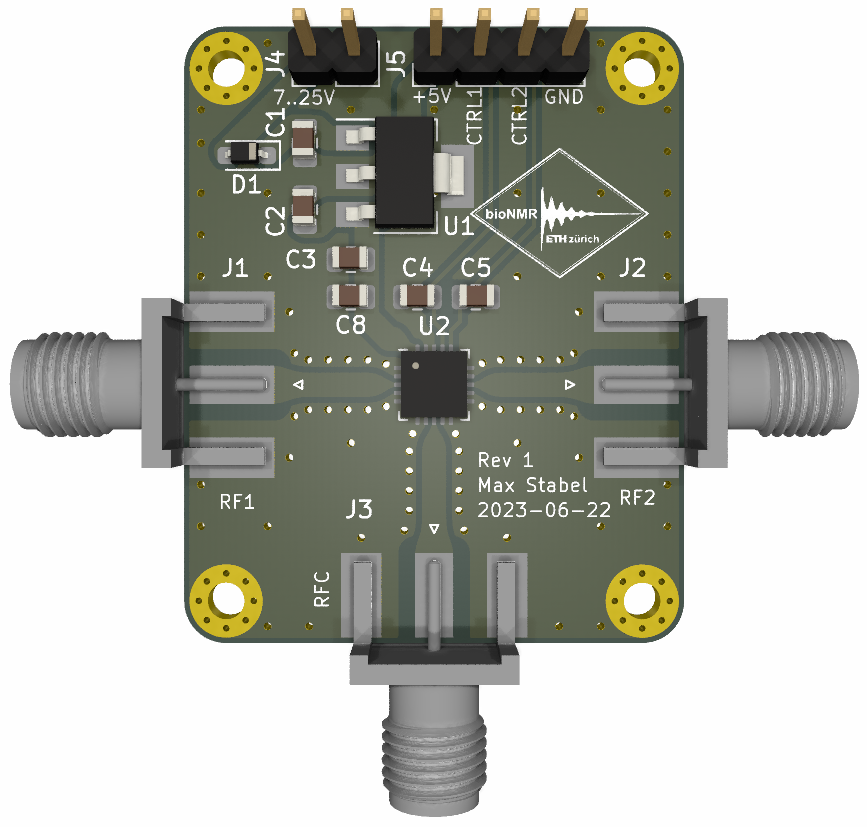
\includegraphics[height=0.9\textheight]{tr_switch.png} \hspace*{5em}
    \begin{tikzpicture}[overlay, remember picture]
        \node[anchor=north east, inner sep=0] (block) at (current page.north east) {\colorbox{white}{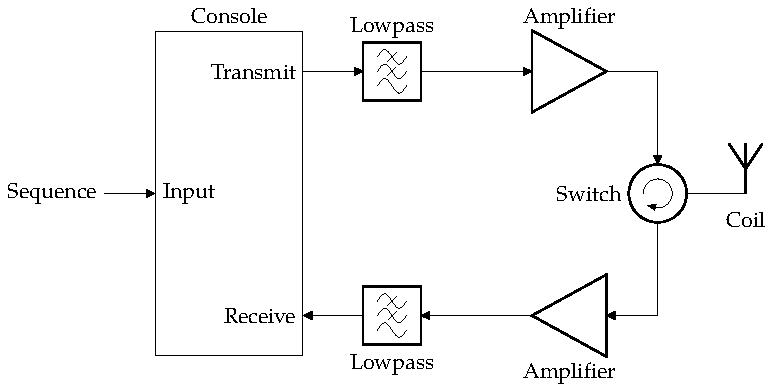
\includegraphics[width=6cm]{block_diagram.pdf}}};
        \draw[red, ultra thick, rounded corners] (block.south west) ++(4.3,1.25) rectangle ++(1.3,0.8);
    \end{tikzpicture}
    \note[item]{Active}
    \note[item]{Isolation: \qty{60}{dB}}
    \note[item]{Silicon-on-insulator (not pHEMT GaAs) i.e. FET tech, not PIN-Diode}
    \note[item]{PIN-Diode switch also possible, but
        \begin{itemize}
            \item usually higher leakage
            \item slower switching
            \item harder to integrate on a chip
            \item but higher power capabilities
        \end{itemize}
    }
\end{frame}


\begin{frame}{The probe}
    % \centering
    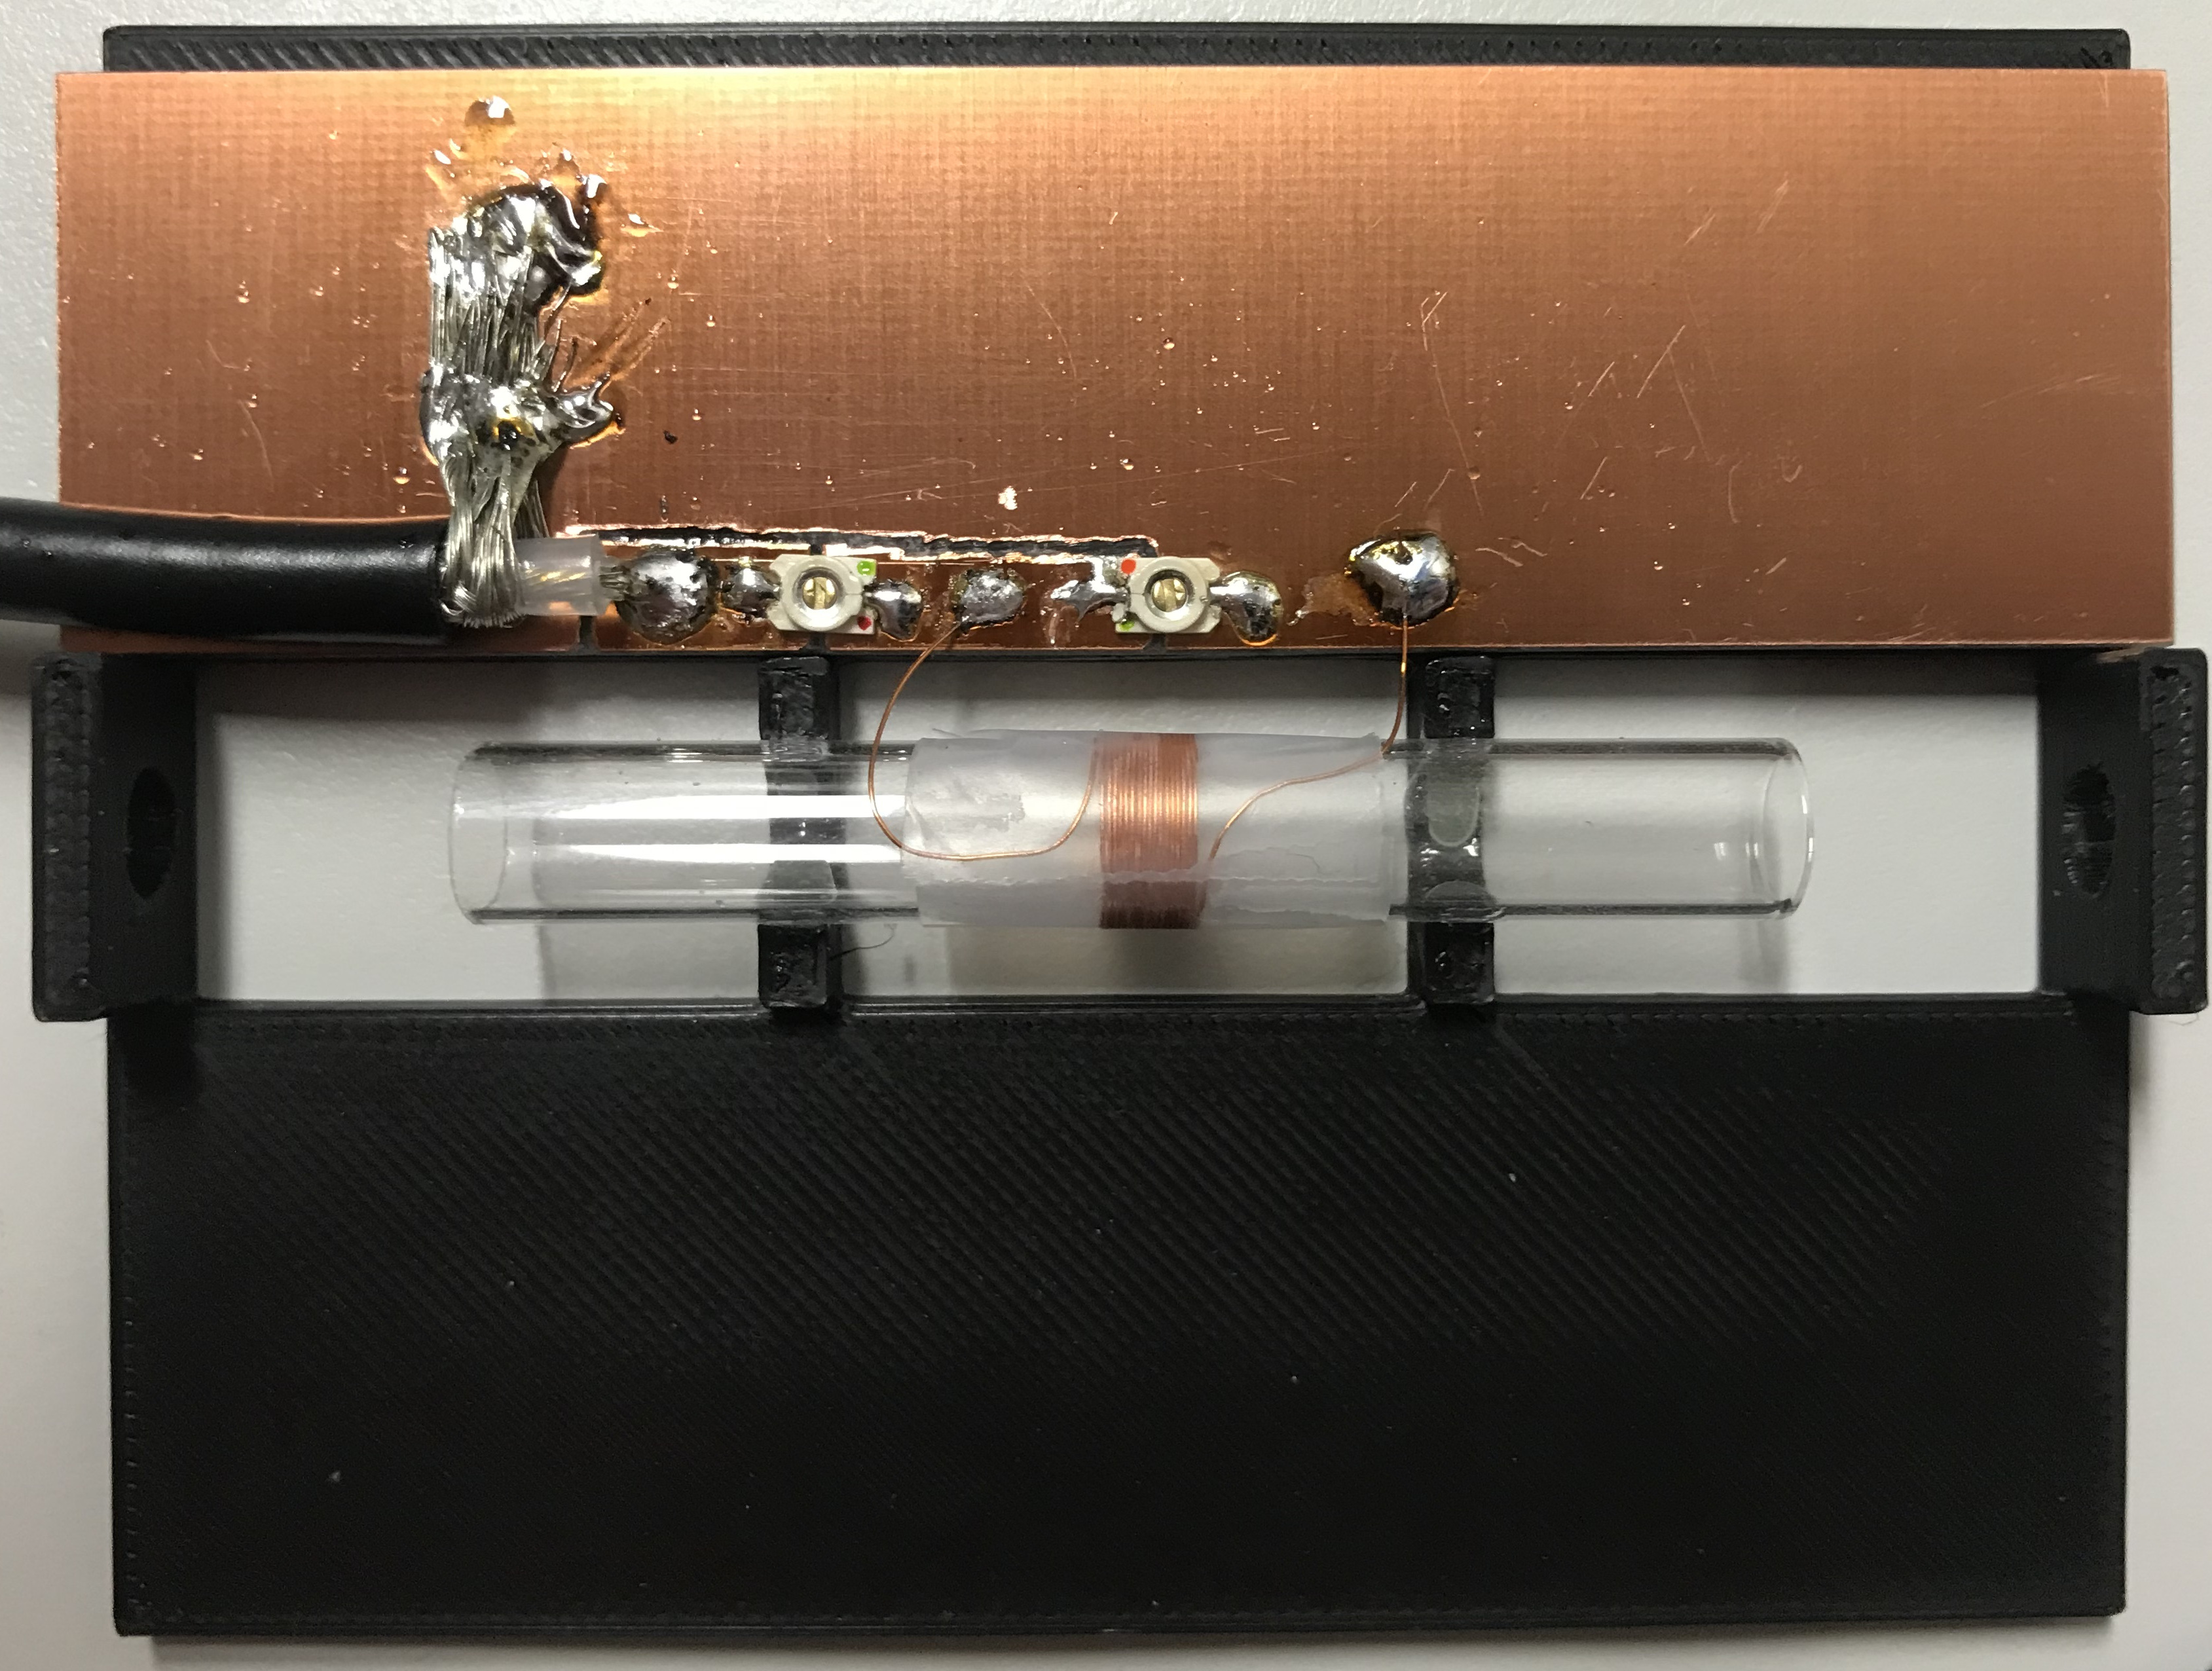
\includegraphics[height=0.8\textheight]{probe.jpg}
    \begin{tikzpicture}[overlay, remember picture]
        \node[anchor=north east, inner sep=0] (block) at (current page.north east) {\colorbox{white}{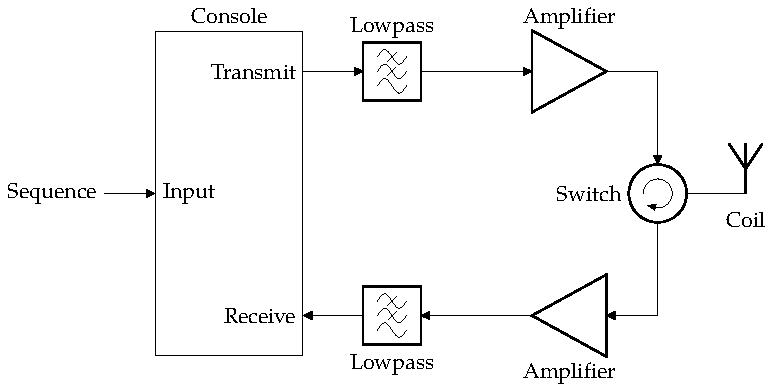
\includegraphics[width=6cm]{block_diagram.pdf}}};
        \draw[red, ultra thick, rounded corners] (block.south west) ++(5.6,1.25) rectangle ++(0.6,1);
    \end{tikzpicture}
    \note[item]{Many turns --- high inductance --- low capacitance --- sensitive to stray capacitance}
\end{frame}

\begin{frame}{A 32-channel current supply is designed but untested}
    \centering
    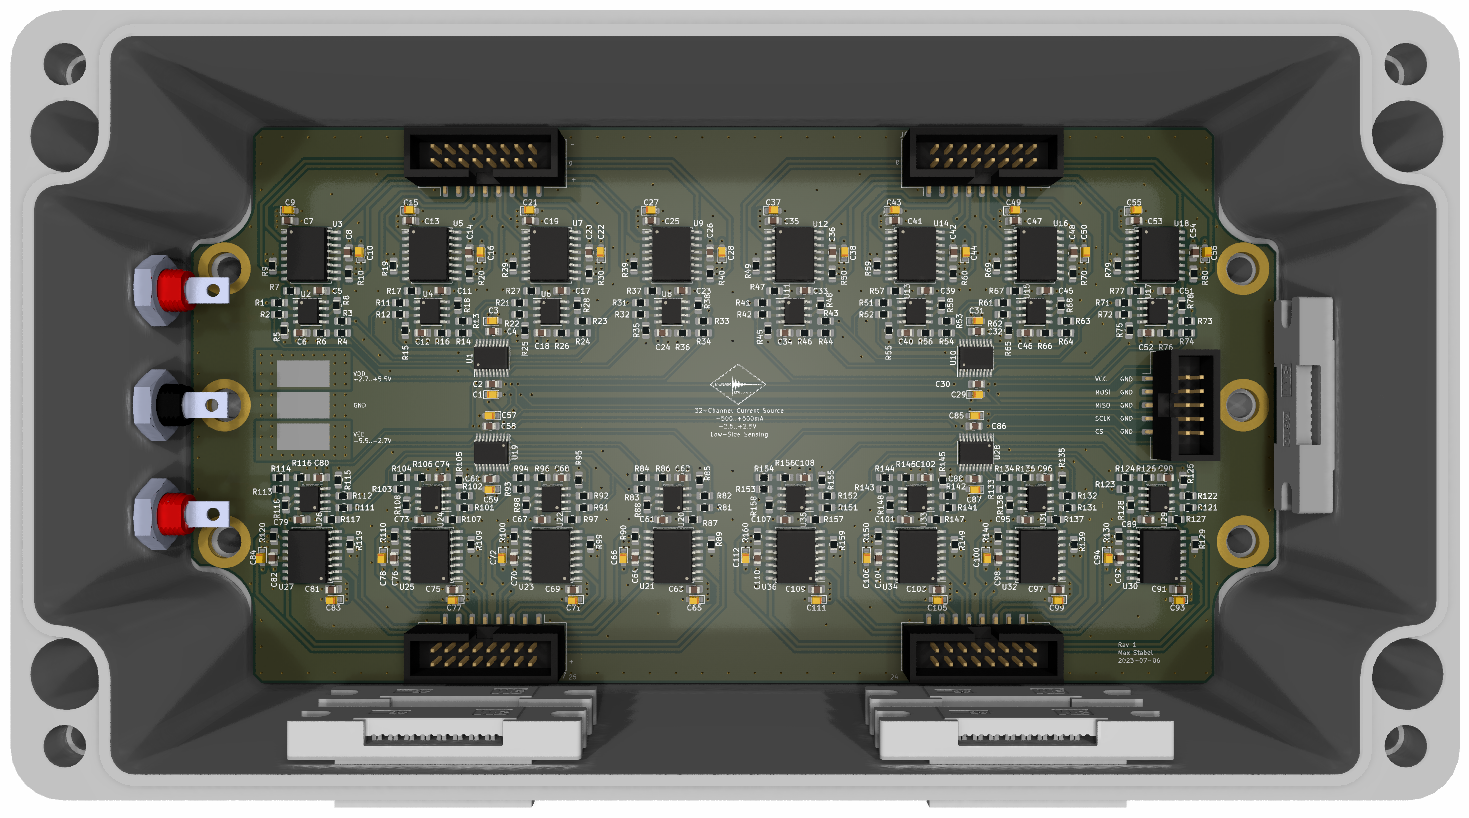
\includegraphics[height=0.8\textheight]{32-channel_current_source.png}
\end{frame}

\section{The complete setup}


\begin{frame}{Our NMR is affordable \ldots}
    \vspace*{-0.5\baselineskip}
    \begin{table}
        \begin{tabular}{@{}
                l
                S[table-format=7.0,table-align-text-pre=false]
                S[table-format=3.2,table-align-text-pre=false]
                S[table-format=5.2,table-align-text-pre=false]
                @{}}
            \toprule
                                & {\qty{600}{\mega\hertz}\footnote{estimated costs}} & {mini-circuits} & {\magnethical}          \\
            \midrule
            Power Amplifier     & 50000                                              & 323.49          & 36.01                   \\
            Switch              & {-}                                                & 82.06           & 20.05                   \\
            Probe               & 100000                                             & {-}             & {\approx} 15.00         \\
            Low-Noise Amplifier & 50000                                              & 409.38          & 73.11                   \\
            Shim Driver         & {-}                                                & {-}             & 257.08                  \\
            Console             & 200000                                             & {-}             & 662.53                  \\
            Magnet              & 1000000                                            & {-}             & {\approx} 9000.00       \\
            \bottomrule
            \textbf{Sum}        &                                                    &                 & \textbf{\num{10142.80}} \\
        \end{tabular}
    \end{table}
    \freefootnote{Prices incl. VAT [CHF]}
\end{frame}

\begin{frame}{\ldots{} competitive \ldots{}}
    \begin{table}
        \begin{tabular}{@{} lrrr @{}}
            \toprule
                                           & Superconducting                        & Benchtop                            & \magnethical{}                                             \\
            \midrule
            Price [k\,CHF]                 & \numrange[range-phrase=--]{200}{18000} & \numrange[range-phrase=--]{50}{150} & \approx\num{10}                                            \\
            Frequency [\unit{\mega\hertz}] & \numrange[range-phrase=--]{300}{1200}  & \numrange[range-phrase=--]{40}{125} & \num{25}                                                   \\
            Resolution [\unit{\hertz}]     & \approx\num{0.2}                       & \numrange[range-phrase=--]{0.2}{1}  & \approx \num{2.5}/\num{50}\footnote[2]{with/without shims} \\
            Weight [\unit{\kilo\gram}]     & \numrange[range-phrase=--]{600}{15000} & \numrange[range-phrase=--]{25}{150} & \approx\num{5}                                             \\
            % \bottomrule
        \end{tabular}
    \end{table}
    \freefootnote{For 5mm standard NMR tubes}
\end{frame}

% Add picture of complete setup
\begin{frame}{\ldots{} and portable}
    \vspace*{-2\baselineskip}
    \centering
    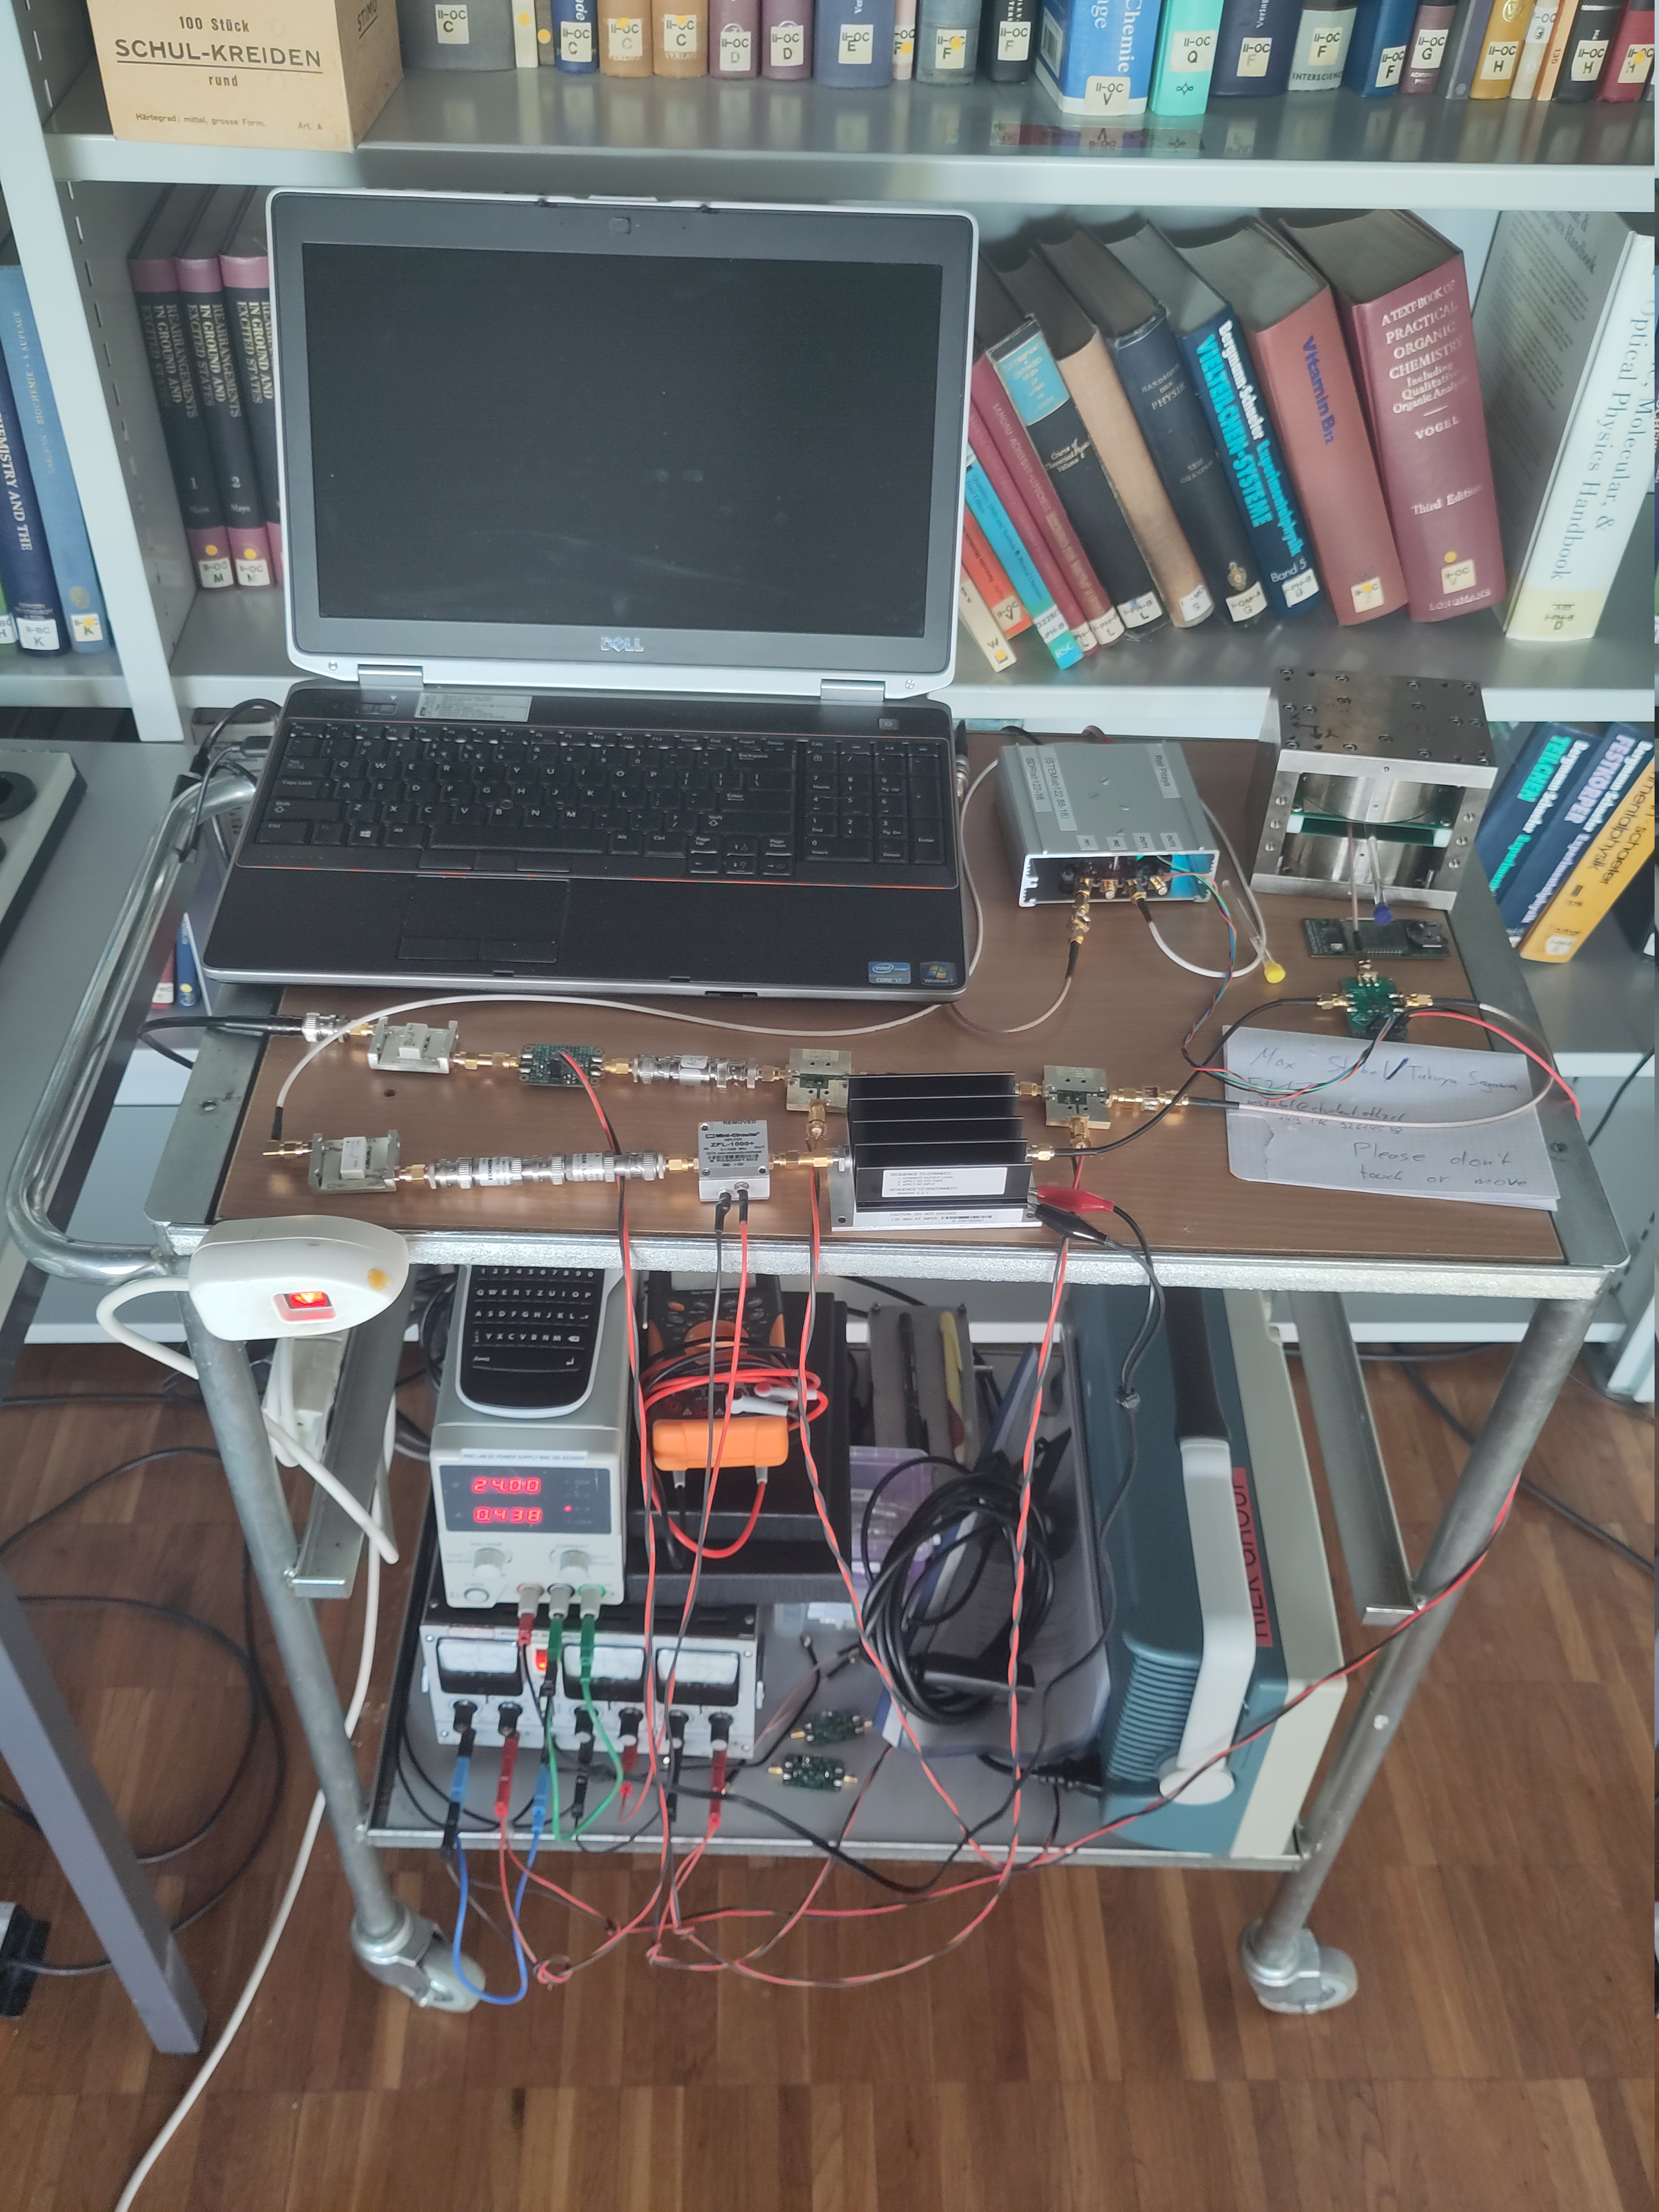
\includegraphics[height=\textheight]{complete_setup.jpg}
\end{frame}

% Results
\section{Experimental Results}

\begin{frame}{Simple Pulse Sequence}
    \centering
    \includesvg[width=0.5\textwidth]{simple_pulse_sequence.svg}
\end{frame}

\begin{frame}{We can already see a water FID}
    \centering
    % \includegraphics[width=0.9\textwidth]{images/fid_sine_fit.pdf}
    % TODO: add T2*
    \begin{tikzpicture}
        \node[anchor=south west,inner sep=0] (image) at (0,0) {
            \includegraphics[width=0.9\textwidth]{fid_sine_fit.pdf}
        };
        \begin{scope}[overlay]
            \node[anchor=east](t2) at (image.north east){\(T_2^* = \qty{2.55}{\milli\second}\)};
        \end{scope}
    \end{tikzpicture}
    \note[item]{Outliers at the beginning are due to CIC filters}
\end{frame}

\begin{frame}{\ldots and do a Fourier transform}
    \centering
    \begin{tikzpicture}
        \node (fft)
        {
            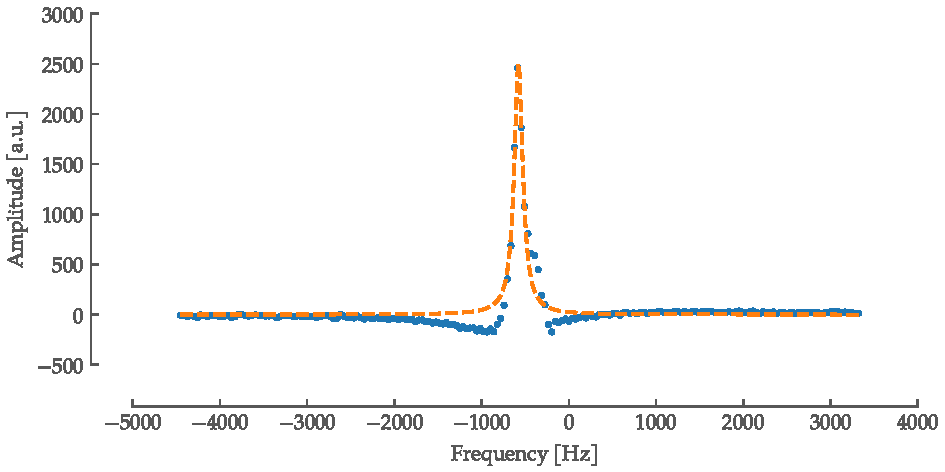
\includegraphics[width=0.9\textwidth]{images/fft_fit.pdf}
        };
        \begin{scope}[overlay]
            \node (structure) at (fft.north)
            [
                anchor=center,
                xshift=0.65cm,
                yshift=0cm
            ]
            {
                \includesvg[height=0.1\textheight]{images/h2o.svg}
            };
            \path[draw=grey,dashed,->] ([yshift=1mm,xshift=-3mm]structure.south east) to ([xshift=0.7cm,yshift=2.5cm]fft.center);
            \path[draw=grey,dashed,->] ([yshift=1mm,xshift=3mm]structure.south west) to ([xshift=0.6cm,yshift=2.5cm]fft.center);
            \node[anchor=north east](label) at (fft.north east){%
                \(
                \begin{aligned}
                    T_2^*       & = \qty{2.71}{\milli\second} \\
                    \text{FWHM} & = \qty{117.7}{\hertz}
                \end{aligned}
                \)
            };
        \end{scope}
    \end{tikzpicture}
    \note[item]{Not Lorentz because of missing shimming/inhomogeneities}
    \note[item]{Measured input signal of -92dBm/15.8uV resulted in amplitude of 2200}
    \note[item]{SNR of around 350, With FWHM 2.5Hz/1ppm we estimate snr of 11000}
\end{frame}

\begin{frame}{Toluene also has a visible signal}
    \centering
    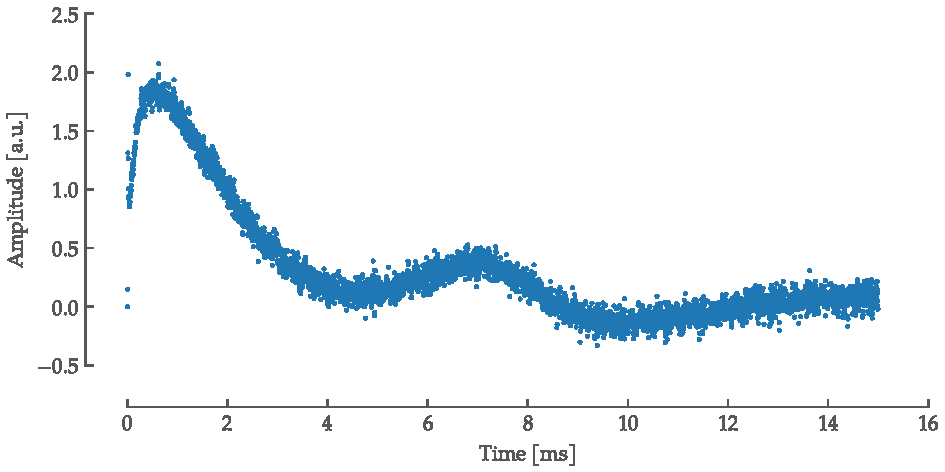
\includegraphics[width=0.9\textwidth]{images/fid_toluene.pdf}
\end{frame}

\begin{frame}{We can even see the chemical shifts\\of the Toluene peaks!}
    \centering
    \begin{tikzpicture}
        \node (fft)
        {
            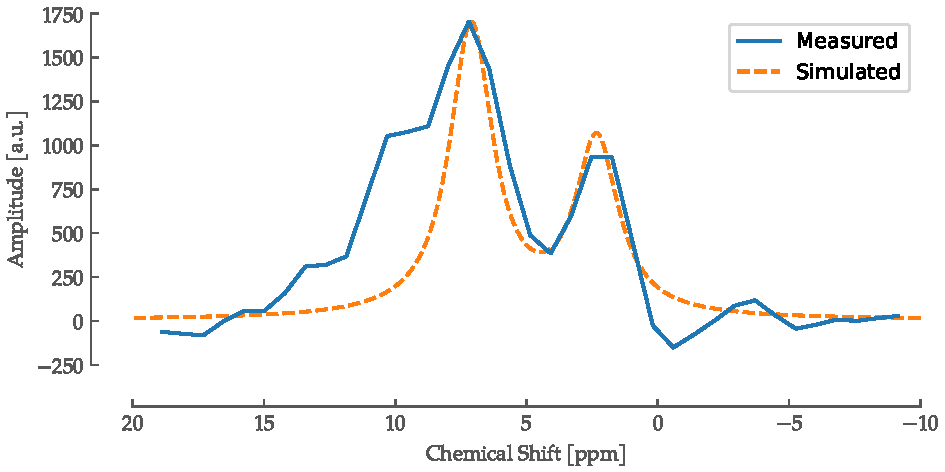
\includegraphics[width=0.9\textwidth]{images/fft_toluene.pdf}
        };
        \begin{scope}[overlay]
            \node (structure) at (fft.north)
            [
                anchor=north west,
                xshift=0mm,
                yshift=1.5cm
            ]
            {
                \includesvg[height=0.15\textheight]{images/toluene.svg}
            };
            \path[draw=grey,dashed,->] ([yshift=5mm,xshift=-4mm]structure.south east) to ([yshift=1.5cm,xshift=1.75cm]fft.center);
            \path[draw=grey,dashed,->] ([yshift=2mm,xshift=2mm]structure.south west) to ([yshift=3.1cm]fft.center);
        \end{scope}
    \end{tikzpicture}
    \note{It's a full tube of toluene, not a solution}
    \note[item]{Reasons for sidepeak: no apodization (truncation of FID), no shimming, inhomogeneities/not centred}
\end{frame}

\begin{frame}{Rabi nutation (pulse calibration) of water}
    \centering
    \begin{tikzpicture}
        \node (rabi)
        {
            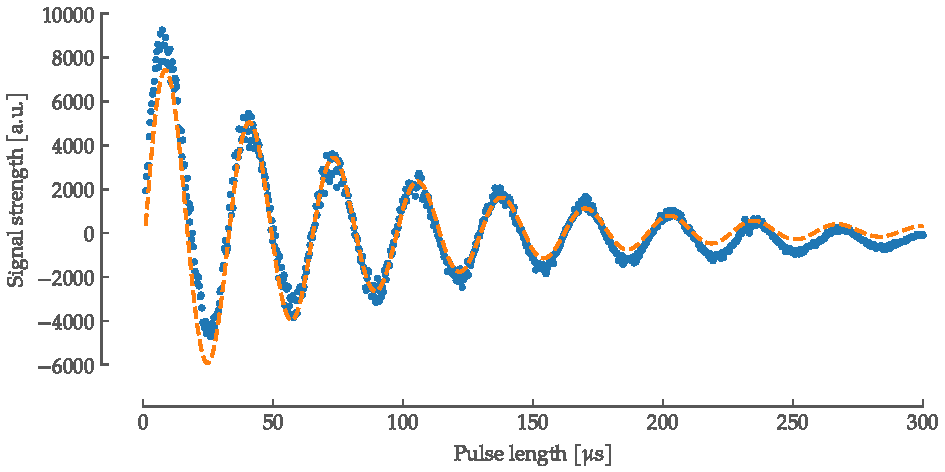
\includegraphics[width=0.9\textwidth]{rabi_nutation_fit.pdf}
        };
        \begin{scope}[overlay]
            \node[anchor=north east](label) at (rabi.north east){%
                \(
                \begin{aligned}
                    2\pi{}          & \mathrel{\hat{=}} \qty{32.3}{\micro\second} \\
                    \frac{\pi{}}{2} & \mathrel{\hat{=}} \qty{8.07}{\micro\second}
                \end{aligned}
                \)
            };
        \end{scope}
    \end{tikzpicture}
    \note[item]{\(T_{period} = \qty{32}{\micro\second}\)}
    \note[item]{\(T_{\frac{\pi}{2}} = \qty{8}{\micro\second}\)}
\end{frame}

\begin{frame}{Spin Echo Sequence}
    \centering
    \includesvg[width=0.9\textwidth]{spin_echo_sequence.svg}
\end{frame}

\begin{frame}{Spin Echo Animation}
    \begin{center}
        \movie[width=8.7cm,height=6.5cm]{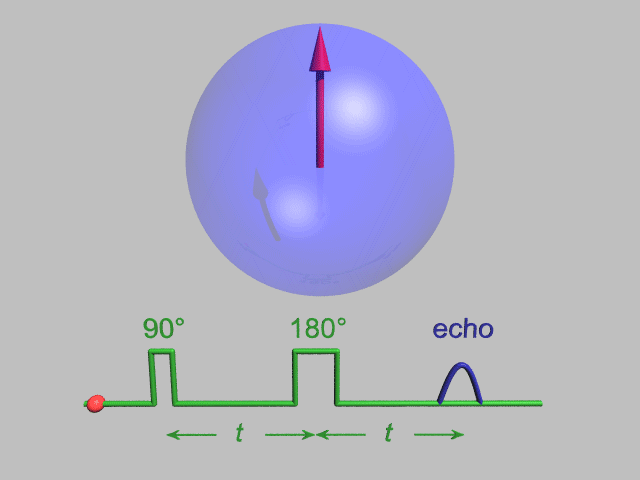
\includegraphics[height=6.5cm,width=8.7cm]{hahn_echo_cc_gwm.png}}{./hahn_echo_cc_gwm.gif}
    \end{center}
    \freefootnote{\href{https://commons.wikimedia.org/wiki/File:GWM_HahnEcho.gif}{Gavin Morley --- CC BY-SA 3.0}}
\end{frame}

\begin{frame}{Spin Echo Measurement}
    \centering
    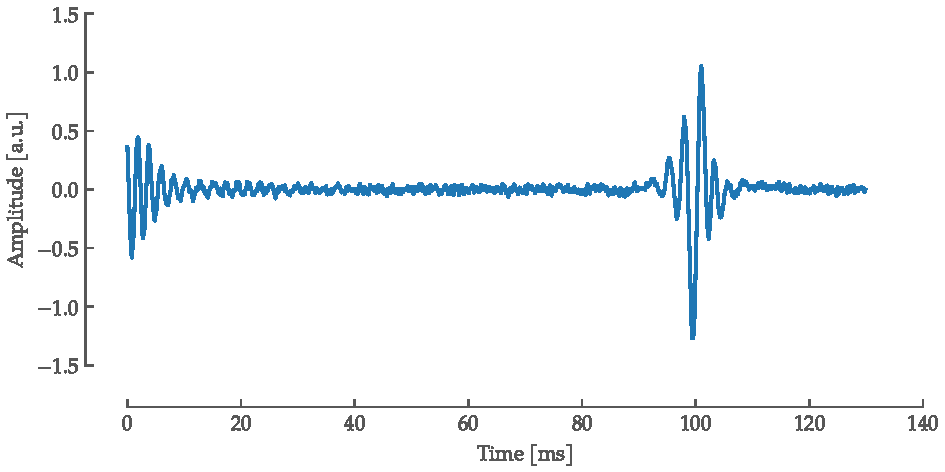
\includegraphics[width=0.9\textwidth]{spin_echo_avg.pdf}
\end{frame}


\begin{frame}{\(T_2\) decay of water}
    \centering
    \begin{tikzpicture}
        \node (decay)
        {
            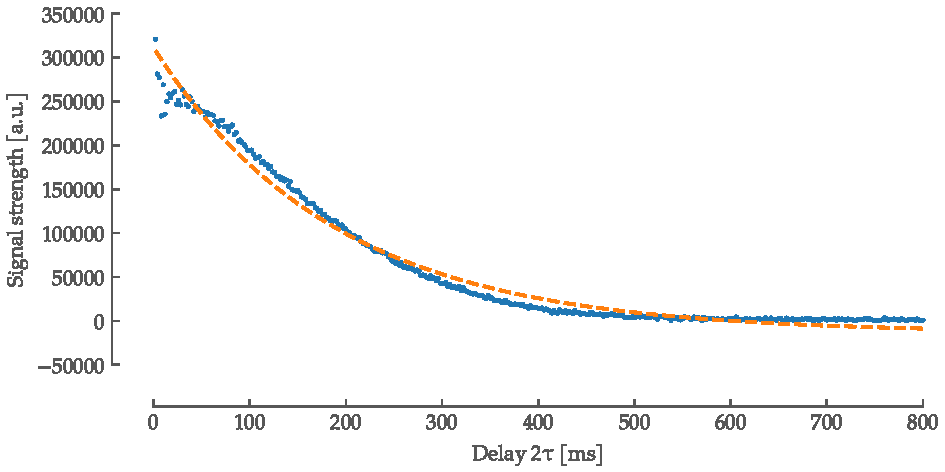
\includegraphics[width=0.9\textwidth]{t2_decay_fit.pdf}
        };
        \begin{scope}[overlay]
            \node[anchor=north east](label) at (decay.north east){\(T_2 = \qty{190}{\milli\second}\)};
        \end{scope}
    \end{tikzpicture}
    \note[item]{\(T_2 = \)}  % Add to slide
\end{frame}

% Demonstration! Measure FID of water/toluene
% TODO: Backup slides with notebook screenshots of measurements
\begin{frame}[standout]
    Demo time!
\end{frame}

% Review
% Conclusion
% Restate main message
% complement with other interpretations 
\begin{frame}{Review}
    \begin{itemize}
        \item Why?
        \item The parts%
              \begin{itemize}
                  \item Console
                  \item Amplifiers
                  \item Switch
                  \item Probe
              \end{itemize}
        \item Capture \& Process Software
        \item Experimental Results
        \item Demonstration
    \end{itemize}
\end{frame}
% We've understood why NMR is desirable
% We've gone through the concept of what it is
% We've step by step built the spectrometer from console, tx, rx, switch and probe
% We've now seen how a the software works and performed a measurement
% I hope I could convince you that the whole setup is working

\begin{frame}{Outlook}
    \begin{itemize}
        \item Shim Driver
        \item Shielding
        \item Improve any part individually%
              \begin{itemize}
                  \item Cheaper Magnet
                  \item Better Probe
                  \item Software (CIC compensation filter, frequency adjustment during pulse, \ldots)
              \end{itemize}
        \item Investigate temperature stability
        \item Sell it to NexMR (or do Photo-CIDNP ourselves)
    \end{itemize}
\end{frame}

% NuevoMR shims, sabr enterprises manget

% Close
\begin{frame}{}
    \begin{center}
        \note[item]{Circling back to the beginning, I would like to end with a quote by E.M. Purcell}
        \emph{
            \enquote{I have not yet lost that sense of wonder, and of delight, that this delicate motion should reside in all ordinary things around us, revealing itself only to him who looks for it.}

            \vspace{2\baselineskip}

            \enquote{There the snow lay around my doorstep --- great heaps of protons quietly precessing in the Earth's magnetic field.}
            % In that on the first snowy, silent night this winter you'll think of the quiet precessions in the earth's magnetic field.
        }
    \end{center}
    \hfill{}--- E.M.\ Purcell
    \note[item]{I wouldn't have thought I would get a glimpse of this wonder that Purcell describes when starting my thesis here, but I'm glad I did.}
    \note[item]{And I hope none of you have lost it yet}
\end{frame}

% End: Show during questions
\begin{frame}{Thank you!}
    \begin{columns}
        \begin{column}{0.5\textwidth}
            \centering
            \includesvg[width=0.5\textwidth]{./images/logo_magnETHical.svg}
        \end{column}
        \begin{column}{0.5\textwidth}
            \centering
            Find everything on \\ \vspace*{\baselineskip}

            \includesvg[width=0.5\textwidth]{./images/gitlab_qrcode.svg}

            \url{https://gitlab.ethz.ch/mstabel/nmr-spectrometer}
        \end{column}
    \end{columns}
\end{frame}


%%%%%%%%%%%%%%%%%%%%%%%%%%%%%%%%%%%%%%%%%%%%%%%%%%%%%%%%%%%%%%%%%%%%%%%%%%%%%%%
% Appendix / Backup Slides
%%%%%%%%%%%%%%%%%%%%%%%%%%%%%%%%%%%%%%%%%%%%%%%%%%%%%%%%%%%%%%%%%%%%%%%%%%%%%%%

\appendix

\begin{frame}[standout]
    Backup
\end{frame}

\begin{frame}{An amplifier is basically just a transistor}
    \centering
    \begin{columns}
        \begin{column}{0.5\textwidth}
            \begin{itemize}
                \item Transistor:\\voltage-controlled current source
                \item \(
                      \begin{aligned}[t]
                          \text{higher voltage} & \rightarrow{} \text{higher current}          \\
                                                & \rightarrow{} \text{higher voltage } V_{R_C} \\
                                                & \rightarrow{} \text{lower voltage } V_{CE}   \\
                                                & \rightarrow{} \text{\ang{180} phase shift}
                      \end{aligned}
                      \)
            \end{itemize}

        \end{column}
        \begin{column}{0.5\textwidth}


            \begin{circuitikz}
                \draw[nodes={align=center}]
                (0,0) node[npn](Q){}
                (Q.B) to[short,-o] ++(-0.5,0) node[left]{\(V_{in}\)}
                (Q.C) to[R,l=\(R_C\),v<=\(V_{R_C}\)] ++(0,2) node[vcc]{\(V_{CC}\)}
                (Q.C) to[short,*-o] ++(1,0) node[right]{\(V_{out}\)}
                (Q.E) node[ground]{}
                ([shift={(0.1,0)}]Q.E) to[open,v_<=\(V_{CE}\)] ([shift={(0.1,0)}]Q.C)
                ;
            \end{circuitikz}
        \end{column}
    \end{columns}
    \note[item]{We want cheap, so using a simple is the obvious first approach}
    \note[item]{Unfortunately there's a lot to do:%
        \begin{itemize}
            \item Input/Output Impedance Matching
            \item Bias Tee
            \item DC coupling
            \item stability calculations
            \item feedback
            \item temperature compensation (current feedback)
        \end{itemize}
    }
    \note[item]{A complete amplifier is quite expensive}
    \note[item]{Solution: Use monolithic (integrated) amplifier}
    \note[item]{Take care of heat dissipation (Class-A)}
\end{frame}

\begin{frame}{The passive approach leaked too much power}
    % TODO remind of why switch
    % zahlen - gefühl - 25mhz -> wellenlänge
    \centering

    \begin{circuitikz}
        \ctikzset{
            diode=empty,
            diodes/scale=0.8
        }
        \draw[nodes={align=center}]

        % tx diodes
        (0,0) node[left]{Transmit} to[short,o-*] ++(1,0) coordinate(tx)
        (tx) -- ++(0, 0.5) to[D] ++(1.5,0) -- ++(0,-0.5)
        (tx) -- ++(0,-0.5) to[D,invert] ++(1.5,0) -- ++(0, 0.5)
        to[short,*-] ++(1,0) coordinate(mid)

        % A/B
        (mid) node[below](A){A}
        (mid) to[short,*-o] ++(0,2) node[above]{Probe}
        (mid) -- ++(3,0) coordinate(b)
        (b) node[above](B){B}

        % rx diodes
        (b) to[short,-*] ++(0,-0.5) coordinate(rx)
        (rx) -- ++(-0.5,0) to[D] ++(0,-1.5) -- ++(0.5,0)
        (rx) -- ++(0.5,0) to[D,invert] ++(0,-1.5) -- ++(-0.5,0)
        to[short,*-] ++(0,-0.5) node[ground]{}

        (b) to[short, *-o] ++(1,0)
        node[right]{Receive}
        ;
        \draw[<->] (A.east |- B.west) -- (B.west);
        \draw ($(A.east|-B.west)!0.5!(B.west)$) node[above]{\(\frac{\lambda}{4}\)};
    \end{circuitikz}

    \note[item]{So called "video feedthrough"}
    \note[item]{Especially noise during reception phase, leaking through turned off amplifier}
    \note[item]{"Traditional" passive design by Lowe and Tarr}
    \note[item]{Leads to distortion of low-power pulses}
    \note[item]{Same design can be used with PIN-Diodes (effectively current-controlled resistor)}
    \note[item]{But PIN Diodes often need higher frequencies (mid MHz), size of intrinsic semiconductor}
\end{frame}

\begin{frame}{A transmission line transforms impedance}
    \begin{columns}
        \begin{column}{0.6\textwidth}
            \centering
            \only<2->{
                \movie[width=0.8\textwidth]{%
                    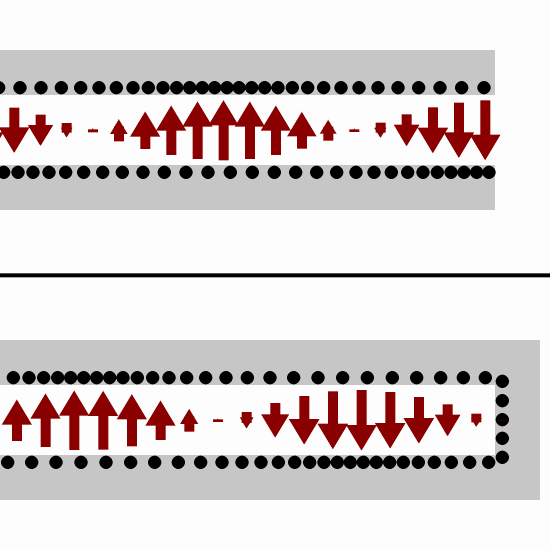
\includegraphics[width=0.8\textwidth]{transmission_line/transmission_line.png}
                }{transmission_line.gif}
            }
        \end{column}
        \begin{column}{0.4\textwidth}
            \vspace*{-0.5cm}

            \begin{circuitikz}
                \draw (0,0) to[short,o-] ++(-3,0) to[vsource,v=\(V_0\)] ++(0,2) to[R,l=\(Z_0\),-o] ++(3,0);
            \end{circuitikz}

            \vspace*{0.75cm}

            \hrule{}

            \vspace*{0.25cm}

            \begin{circuitikz}
                \draw (0,0) to[short,o-] ++(-3,0) to[vsource,v=\(V_0\)] ++(0,2) to[R,l=\(Z_0\),-o] ++(3,0);
                \draw (0,0) to[short,o-] ++(1,0) -- ++(0,2) to[short,-o] ++(-1,0);
            \end{circuitikz}
        \end{column}
    \end{columns}
\end{frame}


\begin{frame}{\(T_2\) Decay Animation}
    \begin{center}
        \movie[width=8.7cm,height=6.5cm]{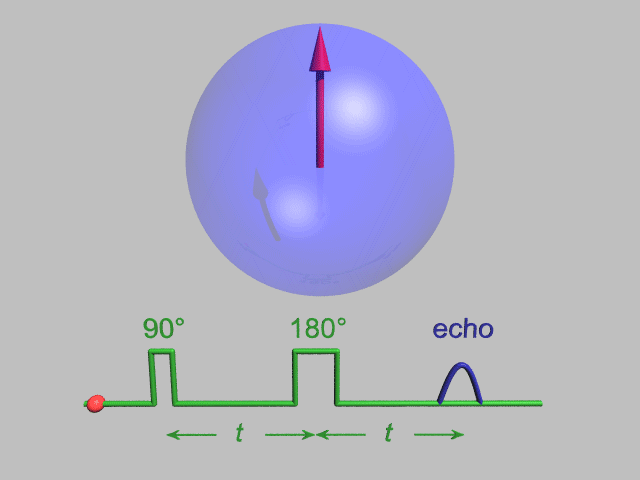
\includegraphics[height=6.5cm,width=8.7cm]{hahn_echo_cc_gwm.png}}{./hahn_echo_decay_cc_gwm.gif}
    \end{center}
    \freefootnote{\href{https://commons.wikimedia.org/wiki/File:GWM_HahnEchoDecay.gif}{Gavin Morley --- CC BY-SA 3.0}}
\end{frame}

\begin{frame}{MaRCoS}
    \centering
    \vspace*{-1\baselineskip}
    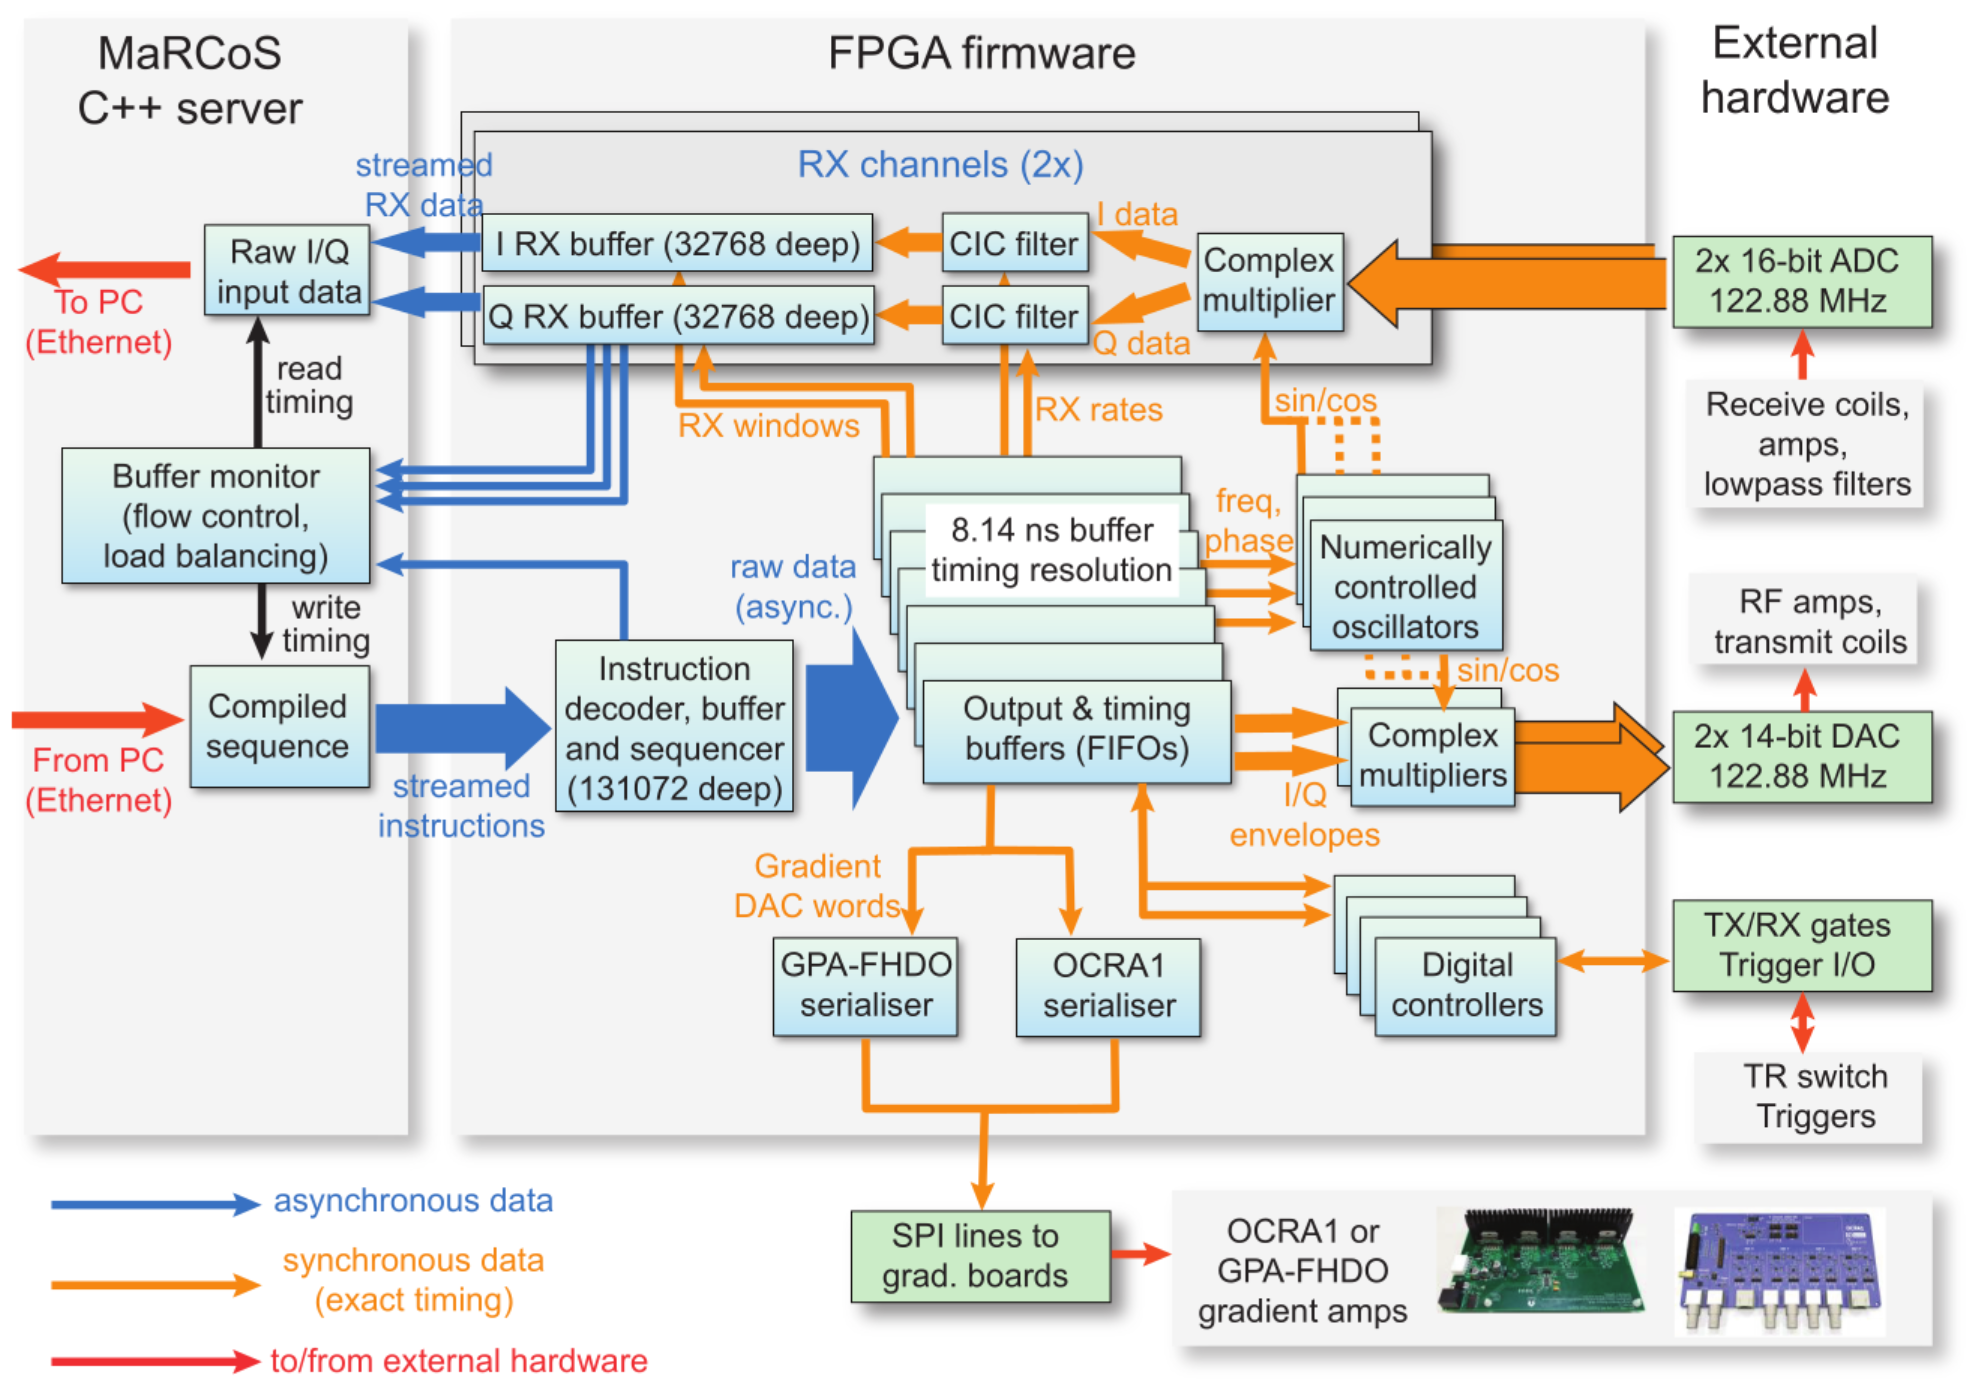
\includegraphics[height=\textheight]{marcos.png}
\end{frame}

\end{document}